\section{Reliability, Recovery, and Long-Running Operations}
\label{sec:reliability}

\begin{designbox}
Treat execution drift --- not weak reasoning --- as the primary risk of a
multi-hour run. Every degradation mode maps to a named guard with an explicit
trigger and action; each guard is task-agnostic, fails soft, and is precise about
whether it may interrupt a live provider call.
\end{designbox}

The reliability model is a set of guards that keep a mission bounded and honest.
Figure~\ref{fig:reliability} sketches how they wrap one Engineer/Reviewer loop.
Table~\ref{tab:guards} is the guard matrix: for each guard, its trigger, its live
default, its action, and --- critically --- whether it can interrupt a call that is
still running. The distinction matters because a guard that severs useful in-flight
work is as harmful as no guard at all.

\begin{figure}[ht]
\centering
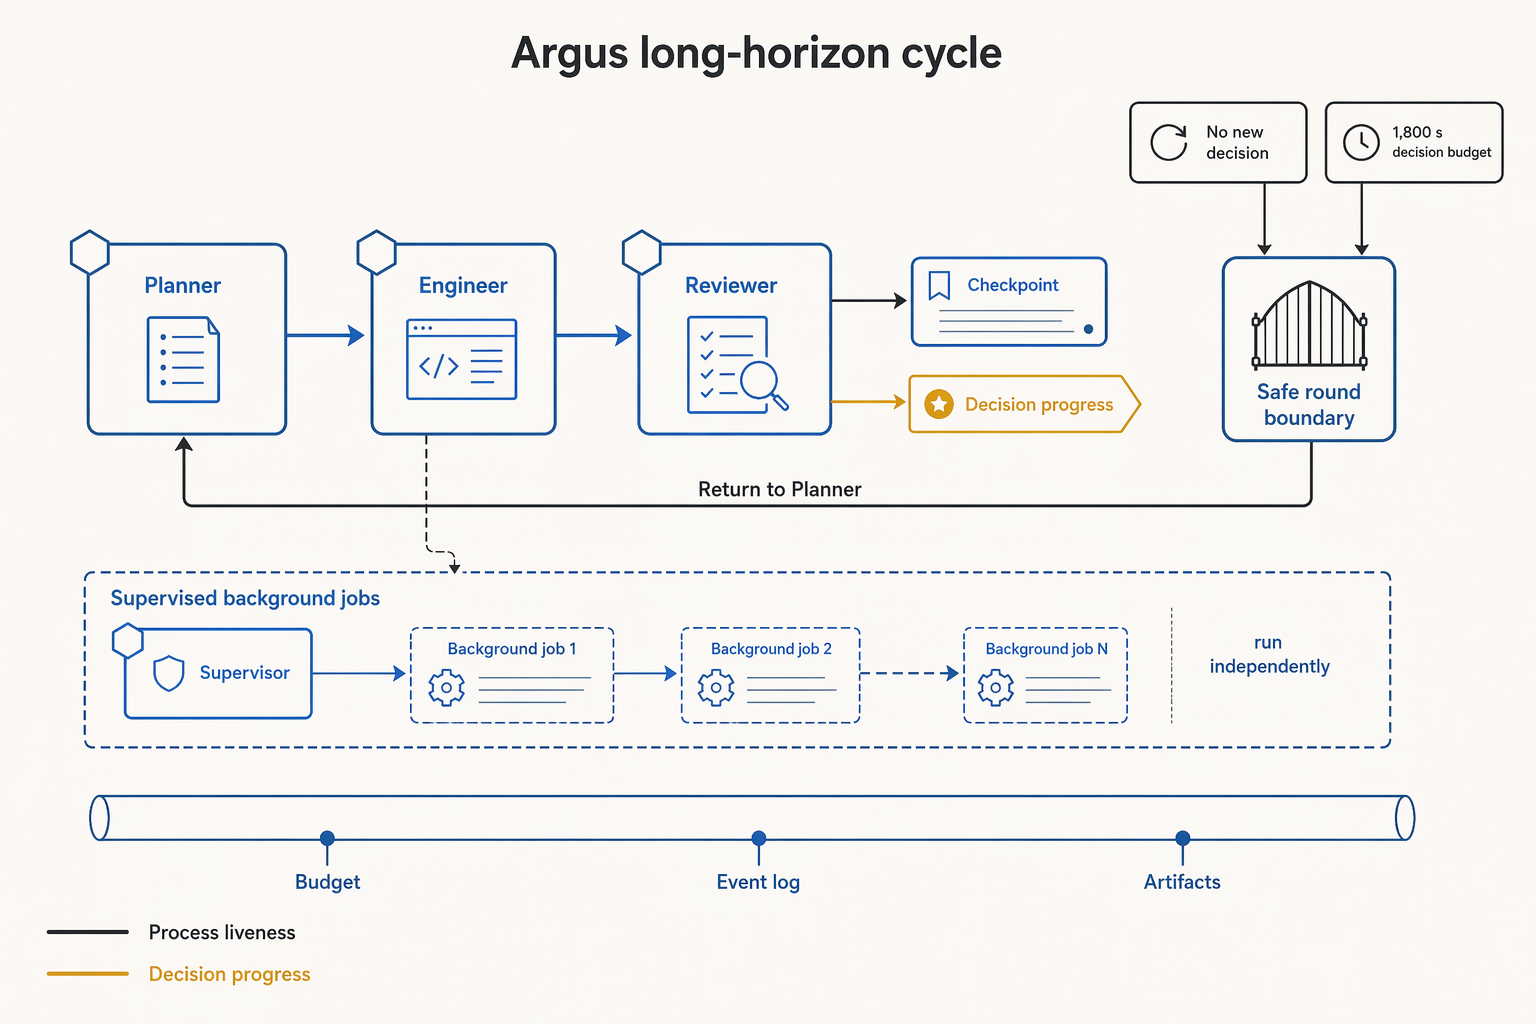
\includegraphics[width=0.6\textwidth]{figures/long_horizon_reliability.png}
\caption{System schematic (not a measured performance plot) of the long-running
reliability cycle: Planner, Engineer, and Reviewer run one loop; the Reviewer
maintains a bounded shared note and a decision-progress class that reseeds a fresh
Engineer thread; supervised background jobs run alongside; and a safe round
boundary returns a stalled or budget-exhausted mission to the Planner, over a
persistent budget, event-log, and artifact rail.}
\label{fig:reliability}
\end{figure}

\subsection{The fault model}

Argus recognizes six recurring fault classes and routes each to a first-class
outcome rather than an unbounded spin. A \emph{provider error or outage} triggers a
bounded backoff and, if it persists, ends the mission as an error (a quota denial
ends it as a paused status, Section~\ref{sec:execution}). \emph{Context pressure} is
defused by fresh-per-round sessions (Section~\ref{sec:state}), with an in-round
compaction guard for the rare repeatedly-compacting round. \emph{Stale or
self-watched jobs} are handled by the background-subagent cadence wait; \emph{no-decision
loops} by counting the Reviewer's \code{progress\_class}; a \emph{reviewer or backend
failure} is treated as infrastructure, never a \code{continue}; and \emph{process
interruption} drains to the mission boundary with an identity-checked resume
(Section~\ref{sec:runtime}).

\subsection{The guard matrix}

\begin{table}[h]
\centering
\small
\begin{tabularx}{\linewidth}{@{}p{2.7cm} X p{1.35cm} p{1.9cm}@{}}
\toprule
\textbf{Guard} & \textbf{Trigger \; / \; action} & \textbf{Default} & \textbf{Interrupts live call?} \\
\midrule
Backend-failure recovery & failure streak $\rightarrow$ backoff, then end as error & 2 / 15\,s & no (round boundary) \\
No-progress bail & consecutive rounds with no engineer message & 2 & no \\
Decision stall & consecutive nondecision \code{progress\_class} rounds $\rightarrow$ end & 2 & no \\
Decision-progress budget & seconds since last decision/evidence $\rightarrow$ end & 1{,}800\,s & \textbf{no} \\
Soft round escalation & round index $\rightarrow$ ask Reviewer to return \code{blocked} & 12 & no \\
Hard round escalation & round index $\rightarrow$ force-end as \code{blocked} & 24 & no \\
Effective-progress watchdog & no file change / non-token event $\rightarrow$ kill subprocess & 3{,}600\,s & \textbf{yes} \\
Runner hard-idle & no runner activity $\rightarrow$ interrupt round & 3{,}600\,s & \textbf{yes} \\
In-round compaction limit & auto-compactions within one round $\rightarrow$ end round & 3 & \textbf{yes} \\
\bottomrule
\end{tabularx}
\caption{Reliability guards (\code{engineer/runner.py}). Round-boundary guards
never sever a live call; the three in-round guards fire only against a subprocess
that is emitting token noise or looping without effective progress. All are
env-overridable and disable at 0.}
\label{tab:guards}
\end{table}

\subsection{Decision progress, not activity}

To separate real progress from busy churn the Reviewer labels each round with a
\code{progress\_class}: \code{decision} or \code{evidence} for genuine forward
motion, or \code{setup\_only}, \code{artifact\_sync\_only}, or \code{none} for
nondecision work. The runtime \emph{counts} these structured labels; it never
infers progress from tool activity, filenames, or token emission. Two consecutive
nondecision rounds trip the stall guard, and the 1{,}800-second decision-progress
budget --- measured from the last decision or evidence increment and checked only
between rounds --- ends a mission that is spinning without ever cutting useful
in-flight work. A separate soft/hard round escalation (12/24) catches the rarer
case of a mission that makes evidence progress every round but never passes its
gate, asking the Reviewer to return \code{blocked} on an external dependency and,
failing that, force-ending so the Planner re-plans.

\subsection{In-round watchdogs}

Three guards operate \emph{inside} a round because they target a subprocess that
has stopped doing useful work. The effective-progress watchdog kills a provider
subprocess that keeps emitting heartbeat or token noise for an hour with no file
change and no non-token session event; the runner hard-idle watchdog interrupts a
round with no runner activity at all; and the in-round compaction guard ends a
round whose session auto-compacts three times (the in-round amnesia-loop
signature). Each default is intentionally long --- research turns legitimately spend
many minutes reading, planning, or waiting on model-side recovery --- and each
disables at 0.

\subsection{Backend-unavailable is infrastructure, not judgment}

A specific, high-cost failure motivated a dedicated path. If the reviewer backend
degrades silently, the sole completion gate can run \emph{blind}: a stale
import-time schema path once caused every reviewer round to exit non-zero, running
the completion gate blind for roughly an hour and a half before it was caught. The
fix routes a backend-unavailable reviewer round to the structured
\code{backend\_unavailable} flag with transport fields, treated as an
infrastructure failure and never as a \code{continue}; the reviewer also preflights
its schema file and raises if it is unreadable rather than proceeding
(\srcpath{reviewer/\_core.py}, \srcpath{core/models.py}). This is the clearest
illustration of the report's reliability posture: the failure was not that a model
reasoned poorly, but that a degraded component was allowed to look healthy.

\subsection{The single anti-stall mechanism}

Layered above the per-round guards is exactly one anti-stuck mechanism,
regime-jump (\srcpath{regime\_jump/}). It \emph{detects} saturation with a simple
counter, \emph{asks} the Planner to judge whether to change regime, and
\emph{enforces} a never-cleared forbidden ledger of exhausted directions --- and it
fails soft to a no-op if anything in the mechanism itself goes wrong. It is a
deliberate choice to have one such mechanism rather than many overlapping
heuristics, each of which would be another place for the infrastructure to
mis-judge the science. None of the guards in this section decides whether the
research is good: each enforces a task-agnostic invariant and fails soft,
preserving the agent's memory and judgment when anything goes wrong --- reliability
is added \emph{around} the agent's judgment, never in place of it.
